\section{Introduction}
%
Large Language Model (LLM) agents solve complex technical tasks by invoking external tools, APIs, and reusable skills \citep{schick2023toolformer, mialon2023augmented}. 
%
As these tools and skills grow from dozens of tools to thousands or even tens of thousands of candidates \citep{patil2023gorilla, li2023apibank, xu2023toolbench, qin2024toolllm}, the core challenge shifts from deciding \emph{whether} to use a skill to retrieving the most relevant set of skills that is sufficient for a task. 
%
\citet{shi2025toolret} already shows that skill retrieval itself is now a major bottleneck in realistic tool ecosystems.

Two common strategies are widely used for handling large skill libraries. 
%
\textbf{Vanilla Skills}~\citep{agentskills2026} prepends the entire skill set to the context window. 
%
This can work for small toolsets, but it scales poorly: token cost grows linearly with library size, and critical domain constraints become easy for the model to overlook inside an overloaded context \citep{liu-etal-2024-lost}.
%\textcolor{red}{cite the paper: lost in the middle}. 
An alternative is \textbf{vector-based retrieval} \citep{lewis2020retrieval, wang2023voyager}, which improves efficiency by retrieving semantically similar skills. 
%
However, semantic proximity does not imply executable sufficiency. In many engineering tasks, the top semantic match is a high-level solver, while the actual solution also requires a lower-level parser, converter, setup utility, or domain-specific preprocessor that is semantically weak but functionally necessary~\citep{qin2024toolllm, liu2025dynamic, patil2023gorilla} (Figure~\ref{fig:prerequisite_gap}).

\begin{figure*}[!t]
    \centering
    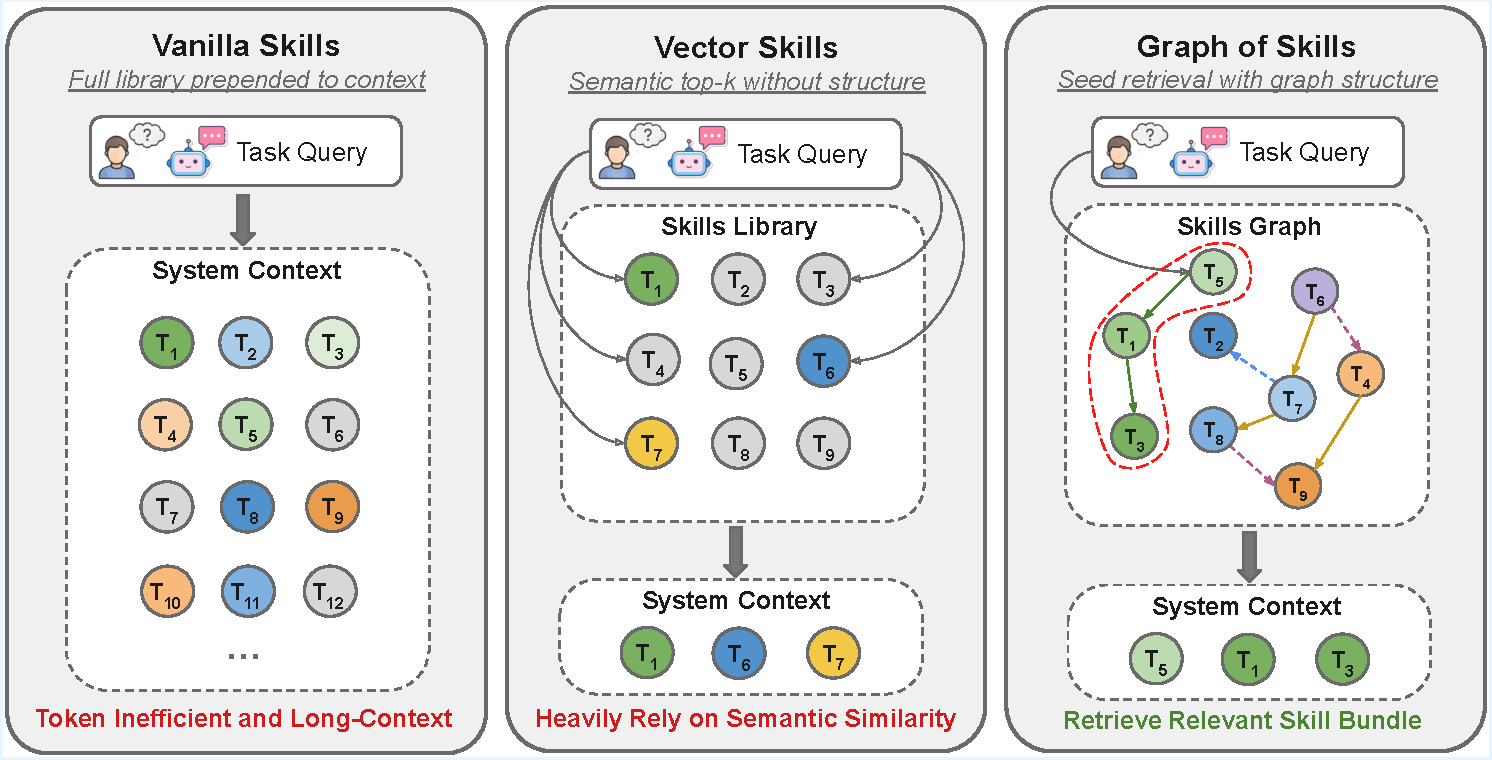
\includegraphics[width=\textwidth]{assests/compare.pdf}
    \caption{Conceptual comparison between flat skill loading, vector retrieval, and Graph-of-Skills (GoS). \textbf{Vanilla Skills} prepends the full skill library to the prompt, so relevant constraints and prerequisite skills become buried in an overloaded context. \textbf{Vector Skills} improves efficiency by returning semantically similar skills, but it can still miss a functionally required prerequisite outside the retrieved set, creating the prerequisite gap. \textbf{Graph-of-Skills} starts from hybrid semantic-lexical seeds and then performs structure-aware retrieval to recover prerequisite skills and assemble a compact execution bundle.}
    \label{fig:prerequisite_gap}
\end{figure*}

% \vspace{-10pt}

We present \textbf{Graph-of-Skills} (GoS), an inference-time structural retrieval layer for large local skill libraries to combat limitations of the previous two approaches. GoS constructs a directed multi-relational graph over local skill packages, where nodes are executable skills and edges encode prerequisite and workflow structure. At query time, GoS uses semantic and lexical signals only to identify a small seed set, then applies reverse-aware Personalized PageRank (PPR)~\citep{10.1145/511446.511513, 10471277} to recover additional skills that are structurally important for execution. The result is a bounded skill bundle that is both relevant and closer to dependency-complete than isolated top-$k$ retrieval.
%
This setting is complementary to repository-scale skill infrastructures such as SkillNet and AgentSkillOS~\citep{skillnet2026, li2026agentskillos}, which focus on creating, organizing, and orchestrating large skill ecosystems. GoS instead targets the downstream question: given an existing local skill library, how should an agent retrieve the smallest executable subset sufficient for the current task? It parses each \skillfile into executable fields, constructs typed dependency and workflow edges, and retrieves a bounded bundle through graph diffusion plus reranking.

Our contributions are as follows:
    % \item We define the \textit{Prerequisite Gap}, a retrieval failure mode in which the semantically obvious skill is found but the executable prerequisite chain is omitted.
    (1) We introduce GoS, an agentic skill usage pipeline that combines offline graph construction with inference-time structural retrieval to improve skill selection accuracy while reducing input token consumption.
    (2) We evaluate GoS across two benchmarks (SkillsBench, ALFWorld) and three model families, and find that on the 1{,}000-skill SkillsBench setting under GPT-5.2 Codex, GoS attains a peak reward gain of 25.55\% over the full skill-loading baseline while reducing total tokens by 56.72\%, with consistent improvement over both baselines in every model--benchmark block. Additional ablations confirm this pattern across skill libraries from 200 to 2{,}000 skills.